%% GENERATED by tools/from_docs.py from stepss-docs. Do not edit by hand:
%% edit the page named below in stepss-docs and regenerate.
%% source: stepss-docs/src/content/docs/models/exciters/basic.mdx

\chapter{Basic exciters}\label{doc:model-exc-basic}

The simplest excitation models: a constant field voltage, a first-order regulator, and the regulator of the Kundur two-area system. \texttt{CONSTANT} and \texttt{1ST\_ORDER} are built in and written in uppercase with no prefix; \texttt{kundur} is registered, and RAMSES adds the \texttt{exc\_} prefix automatically.

The \texttt{EXC} sub-record these models are entered with, and the table of IEEE model variants, are on the \hyperref[doc:model-exc]{Exciter Models} page.

\section{\texorpdfstring{CONSTANT (\texttt{exc\_constant})}{CONSTANT (exc\_constant)}}\label{model-exc-basic:constant-exc_constant}

The data-file model name is \texttt{CONSTANT}.

\subsection{Scientific Description}\label{model-exc-basic:scientific-description}

The \texttt{exc\_constant} model provides a \textbf{constant field voltage} source. The field voltage \(V_f\) is fixed at its load-flow initialisation value and does not respond to any input:

\[V_f(t) = V_{f0} \quad \forall t\]

The single algebraic state satisfies:

\[f(1) = x(1) - V_{f0} = 0\]

This model is useful for open-loop tests, for machines that are not equipped with a voltage regulator, or as a placeholder during model development.

\textbf{Implementation details (from Fortran source):}
- \texttt{nbxvar\ =\ 1}, \texttt{nbzvar\ =\ 0}, \texttt{nbdata\ =\ 0}
- One additional parameter: \texttt{prm(1)\ =\ Vf0} (set at initialisation from the load-flow field voltage)
- Observables: \texttt{vf}, \texttt{if}

\subsection{Parameters}\label{model-exc-basic:parameters}

\begin{small}\begin{longtable}[]{@{}
  >{\raggedright\arraybackslash}p{(\linewidth - 4\tabcolsep) * \real{0.2550}}
  >{\raggedright\arraybackslash}p{(\linewidth - 4\tabcolsep) * \real{0.7450}}
@{}}
\toprule\noalign{}
\begin{minipage}[b]{\linewidth}\raggedright
Parameter
\end{minipage} & \begin{minipage}[b]{\linewidth}\raggedright
Description
\end{minipage} \\
\midrule\noalign{}
\endhead
\bottomrule\noalign{}
\endlastfoot
\emph{(none)} & No user-supplied data parameters. The field voltage is taken from the initialisation (load-flow) value automatically. \\
\end{longtable}\end{small}

\subsection{Usage Example}\label{model-exc-basic:usage-example}

\textbf{RAMSES Data File}

\begin{Verbatim}
SYNC_MACH  GEN1  BUS1
      # FP FQ P Q: share of the power-flow injection (FP, FQ) or initial power (P in MW, Q in Mvar)
      1.  1.  0.  0.
      # SNOM: Nominal apparent power, used as base power in the machine model (MVA)
      600.
      # Pnom: Nominal active power of the turbine, used as base power for the turbine model (MW)
      570.
      # H: Inertia constant (s)
      3.
      # D: Damping coefficient (usually set to zero when the damper windings are modelled) (pu)
      0.
      # IBRATIO: Field current base ratio I_fB^mac/I_fB^exc (see above) (pu)
      0.95
      # TYPE_MOD: Parameter format keyword: RL or XT (case-insensitive)
      XT
      # Xl: Leakage reactance L_l (pu)
      0.15
      # Xd: d-axis synchronous reactance (pu)
      1.1
      # X'd: d-axis transient reactance (must be smaller than Xd) (pu)
      0.25
      # X"d: d-axis subtransient reactance (pu)
      0.2
      # Xq: q-axis synchronous reactance (pu)
      0.7
      # X'q: q-axis transient reactance (pu)
      *
      # X"q: q-axis subtransient reactance (pu)
      0.2
      # m: Saturation coefficient (set to 0 to neglect saturation)
      0.1
      # n: Saturation exponent (ignored when m = 0)
      6.0257
      # Ra: Armature resistance (pu)
      0.
      # T'do: d-axis open-circuit transient time constant (s)
      5.00
      # T"do: d-axis open-circuit subtransient time constant (s)
      0.05
      # T'qo: q-axis open-circuit transient time constant (s)
      *
      # T"qo: q-axis open-circuit subtransient time constant (s)
      0.1
EXC  CONSTANT
TOR  CONSTANT
;
\end{Verbatim}

\textbf{Notes}

\begin{itemize}
\tightlist
\item
  No parameters need to be supplied; the model self-initialises to the load-flow \(V_f\) value.
\item
  Useful for simulation of machines operating in manual excitation mode.
\item
  The model name in the data file is \texttt{CONSTANT} (not \texttt{exc\_constant}).
\end{itemize}

\begin{center}\rule{0.5\linewidth}{0.5pt}\end{center}

\section{\texorpdfstring{1ST\_ORDER (\texttt{exc\_1storder})}{1ST\_ORDER (exc\_1storder)}}\label{model-exc-basic:st_order-exc_1storder}

The data-file model name is \texttt{1ST\_ORDER} (uppercase, with the underscore).

\subsection{Scientific Description}\label{model-exc-basic:scientific-description-1}

The \texttt{exc\_1storder} model is a \textbf{first-order automatic voltage regulator} (AVR). It represents the simplest dynamic exciter: a proportional gain \(K_A\) acting on the terminal voltage error, filtered through a single first-order lag \(T_A\), with output limits.

The AVR computes the voltage error and drives the field voltage:

\[\frac{d V_f}{dt} = \frac{1}{T_A}\left[K_A\left(V_{ref} - V\right) - V_f\right], \quad V_f \in [V_{f,min},\, V_{f,max}]\]

The reference voltage \(V_{ref}\) is initialised from:

\[V_{ref} = V_0 + \frac{V_{f0}}{K_A}\]

\textbf{Implementation details (from Fortran source):}
- \texttt{nbxvar\ =\ 1}, \texttt{nbzvar\ =\ 1}, \texttt{nbdata\ =\ 4}
- Parameters: \texttt{prm(1)\ =\ KA}, \texttt{prm(2)\ =\ TA}, \texttt{prm(3)\ =\ Vfmin}, \texttt{prm(4)\ =\ Vfmax}
- Additional parameter: \texttt{prm(5)\ =\ V0} (voltage setpoint, computed at initialisation)
- The ODE in the continuous mode is:

\[f(1) = \frac{-V_f + K_A(V_{ref} - V)}{T_A}\]

\begin{itemize}
\tightlist
\item
  With anti-windup: if the limiter is active, \texttt{f(1)\ =\ Vf\ -\ Vfmin} (or \texttt{Vfmax}).
\end{itemize}

\begin{figure}[htbp]
\centering
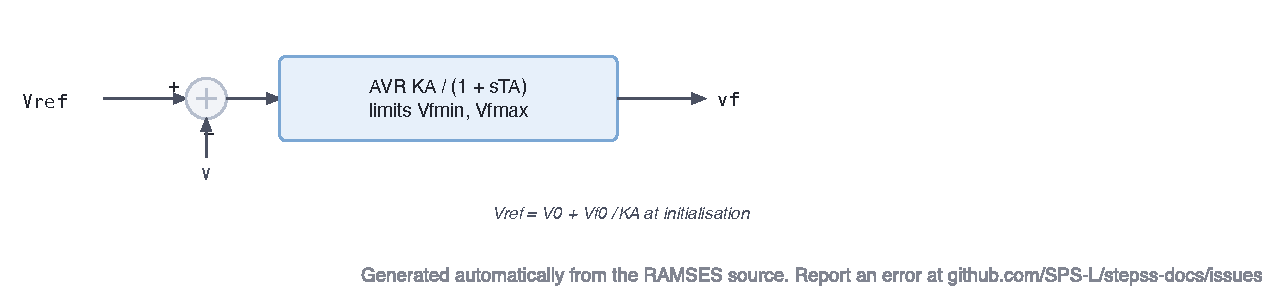
\includegraphics[width=0.98\linewidth]{figures/exc-1storder-light}
\caption{1ST\_ORDER exciter block diagram.}
\end{figure}

\subsection{Parameters}\label{model-exc-basic:parameters-1}

\begin{small}\begin{longtable}[]{@{}ll@{}}
\toprule\noalign{}
Parameter & Description \\
\midrule\noalign{}
\endhead
\bottomrule\noalign{}
\endlastfoot
\texttt{KA} & AVR gain (pu/pu) \\
\texttt{TA} & AVR time constant (s) \\
\texttt{Vfmin} & Minimum field voltage (pu) \\
\texttt{Vfmax} & Maximum field voltage (pu) \\
\end{longtable}\end{small}

\subsection{Usage Example}\label{model-exc-basic:usage-example-1}

\textbf{RAMSES Data File}

\begin{Verbatim}
SYNC_MACH  GEN1  BUS1
      # FP FQ P Q: share of the power-flow injection (FP, FQ) or initial power (P in MW, Q in Mvar)
      1.  1.  0.  0.
      # SNOM: Nominal apparent power, used as base power in the machine model (MVA)
      600.
      # Pnom: Nominal active power of the turbine, used as base power for the turbine model (MW)
      570.
      # H: Inertia constant (s)
      3.
      # D: Damping coefficient (usually set to zero when the damper windings are modelled) (pu)
      0.
      # IBRATIO: Field current base ratio I_fB^mac/I_fB^exc (see above) (pu)
      0.95
      # TYPE_MOD: Parameter format keyword: RL or XT (case-insensitive)
      XT
      # Xl: Leakage reactance L_l (pu)
      0.15
      # Xd: d-axis synchronous reactance (pu)
      1.1
      # X'd: d-axis transient reactance (must be smaller than Xd) (pu)
      0.25
      # X"d: d-axis subtransient reactance (pu)
      0.2
      # Xq: q-axis synchronous reactance (pu)
      0.7
      # X'q: q-axis transient reactance (pu)
      *
      # X"q: q-axis subtransient reactance (pu)
      0.2
      # m: Saturation coefficient (set to 0 to neglect saturation)
      0.1
      # n: Saturation exponent (ignored when m = 0)
      6.0257
      # Ra: Armature resistance (pu)
      0.
      # T'do: d-axis open-circuit transient time constant (s)
      5.00
      # T"do: d-axis open-circuit subtransient time constant (s)
      0.05
      # T'qo: q-axis open-circuit transient time constant (s)
      *
      # T"qo: q-axis open-circuit subtransient time constant (s)
      0.1
EXC  1ST_ORDER
      # KA: AVR gain (pu/pu)
      200.0
      # TA: AVR time constant (s)
      0.05
      # Vfmin: Minimum field voltage (pu)
      0.0
      # Vfmax: Maximum field voltage (pu)
      6.0
TOR  CONSTANT
;
\end{Verbatim}

\textbf{Notes}

\begin{itemize}
\tightlist
\item
  This model is the Fortran-coded equivalent of a simple \texttt{tf1plim} block with input \(V_{ref} - V\).
\item
  \texttt{KA} and \texttt{TA} together set the closed-loop bandwidth.
\item
  The model name in the data file is \texttt{1ST\_ORDER} (uppercase, with the underscore).
\end{itemize}

\begin{center}\rule{0.5\linewidth}{0.5pt}\end{center}

\section{\texorpdfstring{kundur (\texttt{exc\_kundur})}{kundur (exc\_kundur)}}\label{model-exc-basic:kundur-exc_kundur}

The data-file model name is \texttt{kundur} or \texttt{exc\_kundur}. The \texttt{exc\_} prefix is added automatically.

\subsection{Scientific Description}\label{model-exc-basic:scientific-description-2}

The \texttt{exc\_kundur} model implements the \textbf{excitation system from Kundur's textbook} (\emph{Power System Stability and Control}, 1994). It includes a first-order voltage transducer, a proportional AVR with transient gain reduction (TGR), and a two-stage PSS acting on rotor speed deviation.

\textbf{Voltage transducer:}

\[\frac{d V_{fil}}{dt} = \frac{1}{T_R}(V - V_{fil})\]

\textbf{AVR with transient gain reduction (lead--lag):}

\[V_f(s) = K_A \cdot \frac{1 + s T_A}{1 + s T_B} \cdot \left(V_{ref} - V_{fil} + V_s\right)\]

where \(V_{ref} = V + V_f / K_A\) is computed at initialisation and \(V_s\) is the PSS output.

\textbf{PSS (two-stage lead--lag with washout):}

\[x_{wash}(s) = \frac{K_{STAB} \cdot s T_W}{1 + s T_W} \cdot \omega(s)\]

\[V_s(s) = \frac{1 + s T_1}{1 + s T_2} \cdot \frac{1 + s T_3}{1 + s T_4} \cdot x_{wash}(s)\]

This is the standard two-stage phase-compensating PSS structure. The CODEGEN blocks in the \texttt{.txt} file are:

\begin{small}\begin{longtable}[]{@{}lll@{}}
\toprule\noalign{}
Block & CODEGEN type & Function \\
\midrule\noalign{}
\endhead
\bottomrule\noalign{}
\endlastfoot
Voltage filter & \texttt{tf1p} & \(1/(1+sT_R)\) \\
Main summing junction & \texttt{algeq} & \(V_{ref} - V_{fil} + V_s - dv\) \\
AVR (TGR) & \texttt{tf1p1z} & \(K_A(1+sT_A)/(1+sT_B)\) \\
PSS washout & \texttt{tfder1p} & \(K_{STAB} \cdot sT_W/(1+sT_W)\) \\
PSS lead--lag 1 & \texttt{tf1p1z} & \((1+sT_1)/(1+sT_2)\) \\
PSS lead--lag 2 & \texttt{tf1p1z} & \((1+sT_3)/(1+sT_4)\) \\
\end{longtable}\end{small}

\begin{figure}[htbp]
\centering
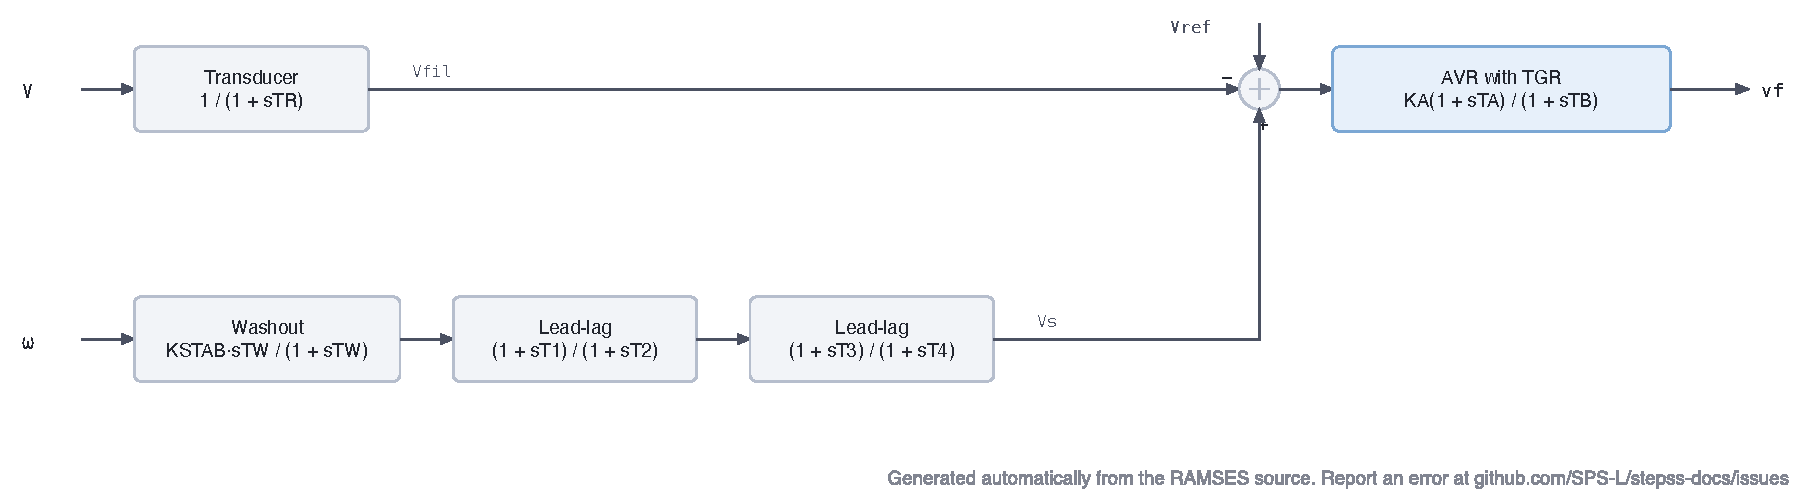
\includegraphics[width=0.98\linewidth]{figures/exc-kundur-light}
\caption{exc\_kundur block diagram.}
\end{figure}

\subsection{Parameters}\label{model-exc-basic:parameters-2}

\begin{small}\begin{longtable}[]{@{}ll@{}}
\toprule\noalign{}
Parameter & Description \\
\midrule\noalign{}
\endhead
\bottomrule\noalign{}
\endlastfoot
\texttt{TR} & Voltage measurement filter time constant (s) \\
\texttt{KA} & AVR gain (pu/pu) \\
\texttt{TA} & TGR lead time constant (s) \\
\texttt{TB} & TGR lag time constant (s) \\
\texttt{KSTAB} & PSS gain \\
\texttt{TW} & PSS washout time constant (s) \\
\texttt{T1} & PSS first lead--lag zero time constant (s) \\
\texttt{T2} & PSS first lead--lag pole time constant (s) \\
\texttt{T3} & PSS second lead--lag zero time constant (s) \\
\texttt{T4} & PSS second lead--lag pole time constant (s) \\
\end{longtable}\end{small}

\textbf{Computed at initialisation:} \texttt{Vref\ =\ V\ +\ Vf\ /\ KA}

\subsection{Usage Example}\label{model-exc-basic:usage-example-2}

\textbf{RAMSES Data File}

\begin{Verbatim}
SYNC_MACH  GEN1  BUS1
      # FP FQ P Q: share of the power-flow injection (FP, FQ) or initial power (P in MW, Q in Mvar)
      1.  1.  0.  0.
      # SNOM: Nominal apparent power, used as base power in the machine model (MVA)
      600.
      # Pnom: Nominal active power of the turbine, used as base power for the turbine model (MW)
      570.
      # H: Inertia constant (s)
      3.
      # D: Damping coefficient (usually set to zero when the damper windings are modelled) (pu)
      0.
      # IBRATIO: Field current base ratio I_fB^mac/I_fB^exc (see above) (pu)
      0.95
      # TYPE_MOD: Parameter format keyword: RL or XT (case-insensitive)
      XT
      # Xl: Leakage reactance L_l (pu)
      0.15
      # Xd: d-axis synchronous reactance (pu)
      1.1
      # X'd: d-axis transient reactance (must be smaller than Xd) (pu)
      0.25
      # X"d: d-axis subtransient reactance (pu)
      0.2
      # Xq: q-axis synchronous reactance (pu)
      0.7
      # X'q: q-axis transient reactance (pu)
      *
      # X"q: q-axis subtransient reactance (pu)
      0.2
      # m: Saturation coefficient (set to 0 to neglect saturation)
      0.1
      # n: Saturation exponent (ignored when m = 0)
      6.0257
      # Ra: Armature resistance (pu)
      0.
      # T'do: d-axis open-circuit transient time constant (s)
      5.00
      # T"do: d-axis open-circuit subtransient time constant (s)
      0.05
      # T'qo: q-axis open-circuit transient time constant (s)
      *
      # T"qo: q-axis open-circuit subtransient time constant (s)
      0.1
EXC  kundur
      # TR: Voltage measurement time constant (s)
      0.02
      # KA: AVR gain (pu/pu)
      200.0
      # TA: Transient gain reduction lead time constant (s)
      0.02
      # TB: Transient gain reduction lag time constant (s)
      10.0
      # KSTAB: PSS gain (pu/pu)
      9.5
      # TW: PSS washout time constant (s)
      1.41
      # T1: PSS first lead-lag numerator time constant (s)
      0.154
      # T2: PSS first lead-lag denominator time constant (s)
      0.033
      # T3: PSS second lead-lag numerator time constant (s)
      0.154
      # T4: PSS second lead-lag denominator time constant (s)
      0.033
TOR  CONSTANT
;
\end{Verbatim}

\textbf{Notes}

\begin{itemize}
\tightlist
\item
  Parameters match the Example 12.6 from Kundur (1994), applicable to a medium-speed generator.
\item
  The PSS stabilises local modes in the 0.5--2 Hz range.
\item
  No output limiter is defined in the base model; add clipping externally if required.
\item
  The model name in the data file is \texttt{kundur} (not \texttt{exc\_kundur}).
\end{itemize}
